\documentclass{article}
\usepackage{graphicx}
\usepackage{geometry}
\usepackage{listings}
\usepackage{hyperref}

 \geometry{
 a4paper,
 total={210mm,297mm},
 left=20mm,
 right=20mm,
 top=20mm,
 bottom=20mm,
 }
 
\begin{document}

\begin{center}
\textbf{\bfseries\Large ASSIGNMENT NO. 4}
\\[1cm]
\end{center}


\section{Aim : } 
	Design suitable mobile app to take a snapshot using mobile camera for Mobile Programming


\section{Objective : }  
	\begin{itemize}
		\item To understand Android Operating System.
		\item To implement Mobile Application Using Android OS.
	\end{itemize}

\section{Software Requirement : }  
	\begin{itemize}
    	\item Java Development Kit (JDK)
		\item Android Studio IDE
		\item Android Operating System
	\end{itemize}

\section{Mathematical Model : }  
	Consider a set S consisting of all elements related to a program. 
	The mathematical model is given as below.  \\  \\
    $S=\{input,output,function,success,failure\}$
	\begin{itemize}
		\item Input  :
			\begin{enumerate}
				\item Select the image
			\end{enumerate}
		\item Output :
        	\begin{enumerate}
				\item Display the selected image
			\end{enumerate}
		\item Function :
			\begin{enumerate}
				\item selectImage()
   				\item displayImage()
			\end{enumerate}
		\item Success : Path to image is valid
        \item Failure : No such situation
	\end{itemize}  

\section{Algorithm : }
	\begin{itemize}
		\item Start
        \item Select the image
        \item Display the selected image
        \item Stop
	\end{itemize}


\section{Theory : }
 	
\subsection{Android:}
	\begin{itemize}
		\item Android is an open source mobile operating system (OS) currently developed by Google, based on the Linux kernel and designed primarily for touchscreen mobile devices such as smartphones and tablets
        \item Android was built from the ground-up to enable developers to create compelling mobile applications that take full advantage of all a handset has to offer. It was built to be truly open
        \item Android has an active community of developers and enthusiasts who use the Android Open Source Project (AOSP) source code to develop and distribute their own modified versions of the operating system
        \item Android provides access to a wide range of useful libraries and tools that can be used to build rich applications. Also includes a full set of tools that have been built from the ground up alongside the platform providing developers with high productivity and deep insight into their applications.
	\end{itemize}
\subsection{Android System Architecture:}
	\begin{figure}[h!]
		\centering
		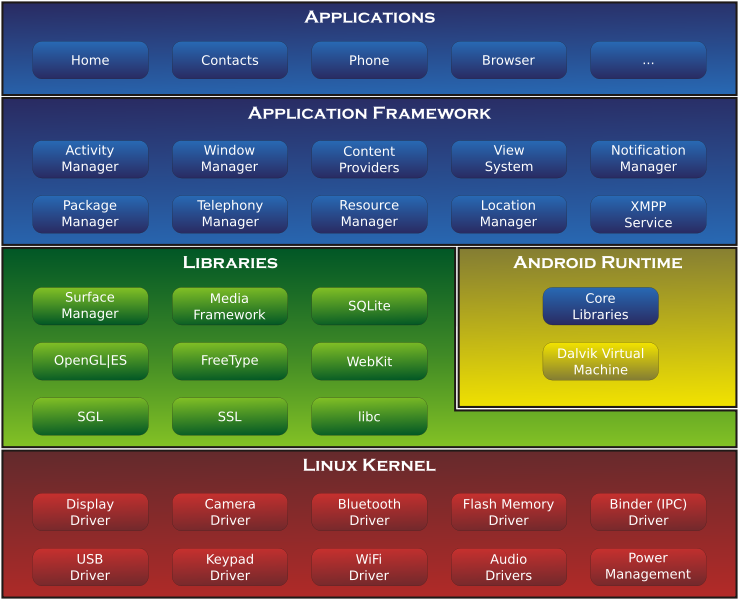
\includegraphics[scale=0.5]{android_architecture.png}
        \caption{Android Architecture}
        \label{fig:android_arch}
	\end{figure}
\subsection{Android Application Development:}    
	\subsection {Creating new project}
    	\begin{itemize}
			\item Open Android Studio
        	\item Select "Create new Android app"
	        \item Set minimum SDK version
	        \item Set the package name for the application
	        \item Select the starting $Activity$
	        \item Finish creating the project
		\end{itemize}  
    \subsection {Android Application Components}
        \begin{enumerate}
        	\item \textbf{Android Manifest}: All the components of the Android application are loosely coupled by the application manifest. It hat describes each component of the application and how they interact.
			\item \textbf{Activity}: An activity represents a single screen with a user interface,in-short Activity performs actions on the screen. For example, an email application might have one activity that shows a list of new emails.
            \item \textbf{Services}: A service is a component that runs in the background to perform long-running operations. For example, a service might play music in the background while the user is in a different application.
            \item \textbf{Broadcast Receivers}: Broadcast Receivers simply respond to broadcast messages from other applications or from the system. For example, applications can also initiate broadcasts to let other applications know that some data has been downloaded to the device and is available for them to use, so this is broadcast receiver who will intercept this communication and will initiate appropriate action.
            \item \textbf{Content Providers}: A content provider component supplies data from one application to others on request. The data may be stored in the file system, the database or somewhere else entirely.
		\end{enumerate} 
        
\subsection{Android - Intent}
	\begin{itemize}
		\item An Intent provides a facility for performing late runtime binding between the code in different applications. Its most significant use is in the launching of activities, where it can be thought of as the glue between activities. It is basically a passive data structure holding an abstract description of an action to be performed.
        \item An Intent is basically a message to say you did or want something to happen. Depending on the intent, apps or the OS might be listening for it and will react accordingly.
	\end{itemize}
    \begin{lstlisting}
     		Intent intent = new
            Intent(android.provider.MediaStore.ACTION_IMAGE_CAPTURE);
    \end{lstlisting}
    \begin{enumerate}
    	\item \textbf{Start activity}:
	    The $startActivityForResult()$ is used to tell $Activity$ that after the 2nd $Activity$ finishes the callback should be returned back to the calling activity
     	\begin{lstlisting}
     		startActivityForResult(intent, 0);
     	\end{lstlisting}
     \item \textbf{Receiving Callback}:
     The $onActivityResult(int requestCode, int resultCode, Intent data)$ is called when once the 2nd $Activity$ finishes is selected.
     	\begin{lstlisting}
     		onActivityResult(int requestCode, 
            int resultCode, Intent data)
     	\end{lstlisting}
     \item \textbf{Intent Action: ACTION\_IMAGE\_CAPTURE}:
     The Standard Intent action that can be sent to have the camera application capture an image and return it. The caller may pass an extra EXTRA\_OUTPUT to control where this image will be written. If the EXTRA\_OUTPUT is not present, then a small sized image is returned as a Bitmap object in the extra field.
	\end{enumerate}


\section{Testing :}

\subsection {Positive / Negative Testing}

\textbf{Positive Testing :}\\
The photo is captured properly and stored into the Gallery.\\

\textbf{Negative Testing :}\\
The photo was not captured due to memory or hardware issues and not stored into the gallery

\section{Conclusion : }

We have successfully developed an Android Mobile Application to capture a snapshot using the Mobile Camera


\end{document}
 
